\documentclass[12pt,a4paper]{article}

\usepackage[margin=2.5cm]{geometry}
\usepackage{times}
\usepackage{amsmath}
\usepackage{amssymb}
\usepackage{graphicx}
\usepackage{booktabs}
\usepackage{array}
\usepackage{tabularx}
\usepackage{caption}
\usepackage{hyperref}
\usepackage{cite}
\usepackage{setspace}
\usepackage{parskip}
\usepackage{float}

\onehalfspacing

\title{\textbf{Multi-Agent AI Framework for Amazon Forest Fire Detection and Spread Forecasting via Satellite Remote Sensing}}
\author{}
\date{}

\begin{document}

\maketitle
\thispagestyle{empty}

% -----------------------------------------------------------------------
\section*{Abstract}
% -----------------------------------------------------------------------

Wildfires in the Amazon rainforest are intensifying each year, threatening biodiversity, indigenous communities, and global climate stability, yet most existing systems detect fires only after significant damage has occurred. In this paper, we propose a multi-agent AI framework that combines satellite remote sensing, machine learning, and large language model (LLM)-based agent coordination to detect fire-prone zones early, simulate how fires would spread, and autonomously plan field response. The system is trained on a 200,000-sample dataset built from six years of INPE fire records, ERA5 weather reanalysis, and live Sentinel-2/MODIS imagery via Google Earth Engine. A LightGBM classifier identifies fire susceptibility with a ROC-AUC of 0.9874 and 95.6\% accuracy. Fire spread is then simulated using a Rothermel physics-based cellular automata model at 100\,m cell resolution, and ecological risk is assessed across 143 protected areas and 351 indigenous territories covering 45,000 grid points. The key novelty is a three-role LLM multi-agent coordination system (Commander, Field Agents, and Evaluator) that autonomously dispatches response teams to intercept the fire front; with six field agents deployed, the system intercepts 54.5\% of the fire front and protects up to 83,031\,ha (30.1\% of the threatened area). These findings highlight the potential of autonomous AI coordination to meaningfully reduce Amazon forest loss and safeguard vulnerable communities.

\medskip
\noindent\textbf{Keywords:} Wildfire Detection, Amazon Rainforest, Satellite Remote Sensing, Multi-Agent Systems, Fire Spread Simulation, Machine Learning, Ecological Risk Assessment

% -----------------------------------------------------------------------
\section{Introduction}
% -----------------------------------------------------------------------

The Amazon rainforest, spanning over 5.5 million square kilometers across nine South American countries, is the largest tropical forest on Earth and a cornerstone of global ecological balance. It absorbs vast quantities of carbon dioxide, regulates regional rainfall patterns, and sustains more than 10\% of all species on the planet. In recent decades, however, this irreplaceable ecosystem has faced an alarming increase in wildfire frequency, driven by prolonged dry seasons, rising temperatures, and widespread deforestation for agricultural expansion. Data from Brazil's National Institute for Space Research (INPE) show tens of thousands of fire occurrences annually across the Brazilian Amazon alone, with peak fire seasons causing widespread destruction of forest cover, displacement of indigenous populations, and measurable spikes in atmospheric carbon emissions. The urgency to develop intelligent, proactive fire management systems for this region has never been greater.

Despite advances in remote sensing technology, existing fire monitoring systems in the Amazon largely operate in a reactive mode, detecting fires only after ignition has already taken place and significant forest area has been lost. Systems such as NASA's FIRMS (Fire Information for Resource Management System) provide near-real-time fire detections from VIIRS and MODIS satellite sensors, but they report confirmed active fires rather than predicting where fires are likely to start or how they will spread once ignited. This fundamental limitation means that emergency response teams are notified too late, with little time to intercept a growing fire front. There is a clear need for systems that can assess fire susceptibility before ignition, forecast how a fire will evolve spatially, and coordinate response resources in a timely and intelligent manner.

Machine learning has shown considerable promise in fire risk prediction, with models trained on meteorological, terrain, and vegetation features achieving strong classification performance. However, most published approaches focus narrowly on binary fire/no-fire prediction and do not extend to spread simulation, ecological impact quantification, or response coordination. In this work, we bridge these gaps by building a modular, end-to-end pipeline. We construct a 200,000-sample training dataset by integrating six years (2018--2023) of INPE fire occurrence records with ERA5 reanalysis weather data and satellite-derived indices, specifically NDVI and NBR from Sentinel-2 and land surface temperature from MODIS, retrieved live via Google Earth Engine. Seven machine learning models are benchmarked, with a LightGBM classifier selected as the production model based on its ROC-AUC of 0.9874 and 95.6\% accuracy on a held-out test set. SHAP and LIME explainability analyses reveal that temperature, humidity, and land cover type are the dominant drivers of fire susceptibility in the Amazon.

Beyond susceptibility prediction, this framework incorporates a physics-based fire spread simulation using the Rothermel rate-of-spread model implemented as a cellular automata on a 51$\times$51 grid of 100\,m cells, capturing the influence of wind direction, terrain slope, fuel type, and fuel moisture on how a fire front evolves over a 12-hour window. A GIS-based ecological risk module then overlays the susceptibility predictions on five boundary layers: 143 federal protected areas, 351 indigenous territories, 130 settlements, 14,785\,km of roads, and 64 river systems, computing vulnerability indices that identify the most at-risk communities and conservation zones across the Brazilian Amazon. Together, these components transform raw satellite observations into actionable, spatially explicit risk intelligence.

The most distinctive contribution of this paper is the introduction of a three-role large language model (LLM) multi-agent coordination system for autonomous fire response planning, comprising a Commander agent, a variable number of Field Agents, and an Evaluator agent. Once a fire spread scenario is generated, the Commander analyzes the threat, prioritizes assets by population and conservation value, and allocates field response teams to interception points along the predicted fire front. Individual Field Agents then verify the feasibility of their assigned routes using a road network graph built from the Amazon highway system, confirming whether they can reach their target before the fire does. The Evaluator agent independently assesses the overall response plan and reports coverage metrics. Evaluated across three deployment scenarios with 2, 4, and 6 field agents respectively, the system demonstrates a clear scaling benefit: six field agents intercept 54.5\% of the fire front and save up to 83,031\,ha of threatened area, underscoring the practical value of autonomous multi-agent coordination in large-scale environmental emergency response.

% -----------------------------------------------------------------------
\section{Related Works}
% -----------------------------------------------------------------------

Recent years have seen a growing body of research applying machine learning, remote sensing, and simulation techniques to wildfire detection, susceptibility mapping, and spread modelling. This section reviews ten closely related works that collectively motivate and contextualise the contributions of the proposed framework.

Xu et al.~\cite{xu2022} proposed LSSVM-CA, a hybrid model that combines least squares support vector machines (LSSVM) with a three-dimensional cellular automata (CA) framework for simulating forest fire spread within a GIS environment. The core motivation was that conventional physical and empirical models struggle to capture the many mutually influencing factors that govern fire spread behaviour. In their approach, the LSSVM is trained on actual local fire data to learn complex CA state-transition rules, and the effect of adjacent wind on directional spread is explicitly incorporated. The simulated fire spread area was cross-compared against the actual extracted fire spread area for validation, and the results showed that LSSVM-CA performs well in reproducing both the spatial extent and probability of fire spread. The authors position their work as an algorithmic alternative to physical models such as FIRETEC and WFDS. Our framework follows the same cellular automata paradigm but embeds Rothermel (1972) physics directly into the transition rules rather than learning them from data, and operates at 100\,m cell resolution across the Brazilian Amazon.

Abdollahi and Pradhan~\cite{abdollahi2023} investigated the application of deep learning combined with Shapley Additive Explanations (SHAP) for wildfire susceptibility prediction in the Gippsland region of Victoria, Australia, the location of some of the country's most severe fire events. Their approach fed three categories of conditioning factors, topographical, land-cover/vegetation, and meteorological, into a deep learning model. SHAP summary plots, dependence plots, and bar charts were then used to rank each factor's contribution and understand the reasoning behind specific predictions. Humidity, wind speed, rainfall, elevation, slope, and the Normalized Difference Moisture Index (NDMI) were identified as the most significant predictors. The authors argued that without XAI interpretation, ML-based fire models remain black boxes that are difficult to trust or act upon in operational settings. This work directly motivates our use of SHAP TreeExplainer and LIME within the proposed framework.

Hang et al.~\cite{hang2024} presented a stacked ensemble machine learning approach combined with XAI for forest fire susceptibility mapping in the Nainital district of the Western Himalaya. Their methodology integrated four base models, AdaBoost, Gradient Boosting Machine, XGBoost, and Random Forest, with a Deep Neural Network as the meta-model in a stacking framework. The stacking ensemble and XGBoost achieved ROC-AUC values above 0.90, with XGBoost reaching an AUC of 0.94. SHAP was used to analyse global variable importance, revealing annual rainfall and evapotranspiration as dominant drivers, while LIME provided local instance-level explanations. Our framework adopts a similar multi-model benchmarking and stacking strategy across seven classifiers, with LightGBM selected as the production model.

Iban and Aksu~\cite{iban2024} developed a SHAP-driven XAI framework for wildfire susceptibility mapping in Izmir Province, T\"{u}rkiye. Their study used freely available MODIS Active Fire Collection 6 MCD14ML product pixels as ground truth fire labels, and incorporated fifteen conditioning factors spanning topography, climate, anthropogenic influences, and vegetation characteristics. Three machine learning classifiers, Random Forest, XGBoost, and LightGBM, were trained and evaluated. Random Forest outperformed the other two models, achieving the highest test accuracy of 95.6\%. The agreement between these findings and our own SHAP analysis, where temperature and humidity are the top predictors in the Amazon, reinforces the cross-regional validity of these features.

Rub\'{i} et al.~\cite{rubi2023} applied machine learning to predict the spread behaviour of wildfires in the Brazilian Federal District within the Cerrado biome. A dataset was compiled from Brazilian governmental open data, incorporating climate observations from five monitoring stations, two decades of satellite fire records, NDVI, topographic features, and urbanisation index. AdaBoost achieved 91\% accuracy in predicting the affected wildfire area, outperforming Random Forest (88\%), ANN (86\%), and SVM (81\%). This study is one of the few focused on Brazilian biomes and wildfire spread prediction, making it a direct precedent for our Amazon-scale spread forecasting approach.

Tang et al.~\cite{tang2024} developed a binary machine learning classifier for a forest fire warning system in Thailand. Data covering fire occurrences from January 2019 to October 2022 were acquired from satellite sources via Google Earth Engine. XGBoost was the top-performing model, achieving 99.6\% accuracy and a ROC-AUC of 0.939. Our framework similarly uses GEE as the satellite data backbone and relies on gradient-boosted tree models, confirming the applicability of this architecture across diverse geographic contexts.

Luz et al.~\cite{luz2022} proposed a fully unsupervised methodology for mapping fire susceptibility in the Brazilian Amazon forests. The approach combined multitemporal remote sensing images from Landsat-8 and MODIS, derivative spectral indices, and time-varying anomaly detection, without requiring any labelled training data. While this study shares our geographic scope, its unsupervised character limits its ability to incorporate meteorological and terrain co-variates. Our supervised framework addresses this by fusing live satellite indices, weather data, and terrain features within a labelled training pipeline.

Perello et al.~\cite{perello2024} applied the PROPAGATOR cellular automata-based wildfire simulator to the Liguria region of Italy for the design of prescribed fire plans. PROPAGATOR was first validated on the most significant historical fire event in Liguria in 2022, then used to identify optimal areas for prescribed burns. A Monte Carlo simulation framework was employed to evaluate efficacy under varying fuel loads, ignition conditions, and meteorological patterns. The study demonstrates that CA-based simulators can function as practical operational decision-support tools, the same role our Rothermel-CA engine plays by generating fire front predictions that feed the LLM-based response coordination layer.

Freitas et al.~\cite{freitas2024} used machine learning to map forest fire susceptibility within the Triunfo do Xingu Environmental Protection Area in the Brazilian Amazon. Random Forest and XGBoost models achieved R$^2$ = 0.99. The resulting susceptibility map showed that 39\% of the conservation unit falls in high or very high susceptibility zones. The most important predictors were precipitation, distance from inhabited areas, and land use type. This Amazon-specific study directly supports our use of tree-based ensemble models for susceptibility scoring across the Legal Amazon.

De Santana et al.~\cite{desantana2024} used the maximum entropy (Maxent) method to analyse current Amazon wildfire dynamics and project future fire niches under two contrasting climate scenarios for 2020--2040. The model performed strongly, with AUC values consistently above 0.85. Distance to farming areas was the single most important predictor (53.4\% contribution), indicating that human land-use activities dominate Amazon fire patterns more than climatic variables alone. The baseline model found that 26.5\% of the Amazon already has moderate to very high fire propensity, concentrated in the Arc of Deforestation. These geographic and driver findings are directly consistent with the spatial risk patterns produced by our framework.

% -----------------------------------------------------------------------
\section{Methodology}
% -----------------------------------------------------------------------

This section describes the end-to-end pipeline of the proposed framework, covering dataset construction, fire susceptibility modelling, physics-based spread simulation, ecological risk assessment, and multi-agent response coordination. Figure~\ref{fig:system} presents the overall system block diagram.

\begin{figure}[H]
  \centering
  
\includegraphics[width=0.85\textwidth]{fig1_system_block_diagram.png}
  \caption{System block diagram}
  \label{fig:system}
\end{figure}

\subsection{Dataset Construction and Feature Engineering}

The training dataset is constructed by integrating three independent data sources across the Brazilian Amazon bounding box (Lat: $-12°$ to $+6°$, Lon: $-75°$ to $-50°$) covering the years 2018--2023. Fire occurrence labels are derived from the Brazilian National Institute for Space Research (INPE) annual fire detection CSVs, with confirmed detections assigned a binary label \textit{fire} = 1. An equal number of background (non-fire) points are sampled uniformly across the same spatial and temporal domain to maintain a 50/50 class balance, yielding approximately 200,000 samples in total. Five meteorological features, temperature, relative humidity, precipitation, wind speed, and wind direction, are matched to each point via nearest-neighbour lookup against ERA5 reanalysis NetCDF files. Three satellite-derived spectral indices are retrieved live via Google Earth Engine using the Sentinel-2 SR Harmonized collection (30-day median composite, cloud fraction $<$ 40\%) and the MODIS MOD11A2 8-day product:

\begin{equation}
\text{NDVI} = \frac{B_8 - B_4}{B_8 + B_4}, \qquad \text{NBR} = \frac{B_8 - B_{12}}{B_8 + B_{12}}
\end{equation}

where $B_4$, $B_8$, and $B_{12}$ are Sentinel-2 surface reflectance bands at 665\,nm, 842\,nm, and 2190\,nm respectively. Land surface temperature (LST) is extracted from MODIS MOD11A2 and converted to Celsius. Terrain features, elevation, slope, and aspect, are derived from SRTM and imputed via KDTree nearest-neighbour. Land cover is obtained from MapBiomas Collection~9 and one-hot encoded into five classes. For operational inference, weather values at arbitrary grid points are spatially interpolated from 120 anchor stations using inverse distance weighting (IDW):

\begin{equation}
\hat{f}(x) = \frac{\displaystyle\sum_{i=1}^{k} w_i f_i}{\displaystyle\sum_{i=1}^{k} w_i}, \qquad w_i = \frac{1}{d(x,\, x_i)^2}
\end{equation}

where $f_i$ is the weather value at anchor $x_i$, $d(x, x_i)$ is the great-circle distance, and $k = 6$ nearest anchors are used. The final dataset contains 19 leakage-free features across 200,000 samples.

\begin{table}[H]
\centering
\caption{Dataset Feature Summary}
\label{tab:dataset}
\begin{tabularx}{\textwidth}{lllXX}
\toprule
\textbf{Feature} & \textbf{Source} & \textbf{Type} & \textbf{Mean / Categories} & \textbf{Notes} \\
\midrule
temperature\_c       & ERA5         & Continuous & 27.4°C          & Dominant SHAP predictor \\
humidity\_pct        & ERA5         & Continuous & 74.2\%          & 2nd SHAP predictor \\
precipitation\_mm    & ERA5         & Continuous & 4.1 mm/day      & \\
wind\_speed\_ms      & ERA5         & Continuous & 2.3 m/s         & \\
wind\_direction\_deg & ERA5         & Continuous & 0--360°         & \\
NDVI                 & Sentinel-2   & Continuous & 0.52            & Vegetation greenness \\
NBR                  & Sentinel-2   & Continuous & 0.31            & Burn ratio \\
LST\_celsius         & MODIS        & Continuous & 29.8°C          & Land surface temp \\
elevation\_m         & SRTM         & Continuous & 248 m           & \\
slope\_deg           & SRTM         & Continuous & 3.1°            & \\
aspect\_deg          & SRTM         & Continuous & 0--360°         & \\
land\_cover\_group   & MapBiomas    & Categorical & 5 classes       & One-hot encoded \\
month                & INPE/ERA5    & Ordinal    & 1--12           & Seasonality \\
fire (label)         & INPE         & Binary     & 0 / 1           & 50/50 balance \\
\bottomrule
\end{tabularx}
\end{table}

\begin{figure}[H]
  \centering
  
\includegraphics[width=\textwidth]{fig2_dataset_samples.png}
  \caption{INPE fire occurrence locations across the Amazon bounding box (2018--2023), colour-coded by LightGBM predicted risk class.}
  \label{fig:dataset}
\end{figure}

\subsection{Fire Susceptibility Modelling and Explainability}

Seven machine learning classifiers are trained on an 80/20 stratified train-test split: Random Forest (300 trees), XGBoost, LightGBM, CatBoost, TabNet, a multilayer perceptron (ANN/MLP with hidden layers of 128--64--32 units), and a stacked ensemble. The stacked ensemble combines XGBoost, LightGBM, CatBoost, and TabNet as base models, with a logistic regression meta-learner trained on their out-of-fold probability predictions:

\begin{equation}
\hat{p}_{\text{stack}}(x) = \sigma\!\left(\beta_0 + \sum_{j=1}^{M} \beta_j \hat{p}_j(x)\right)
\end{equation}

where $\hat{p}_j(x)$ is the fire probability output of base model $j$, $\sigma(\cdot)$ is the sigmoid function, $\beta_j$ are the meta-learner weights, and $M = 4$. LightGBM is selected as the production model based on its ROC-AUC of 0.9874 and accuracy of 95.6\% on the held-out test set.

To ensure interpretability, SHAP (SHapley Additive Explanations) values are computed for every prediction using a TreeExplainer. The SHAP value for feature $i$ on instance $x$ is defined as:

\begin{equation}
\phi_i(x) = \sum_{S \subseteq F \setminus \{i\}} \frac{|S|!\,(|F|-|S|-1)!}{|F|!} \left[ f(S \cup \{i\}) - f(S) \right]
\end{equation}

where $F$ is the full feature set, $S$ is a feature subset, and $f(S)$ is the model output using only features in $S$. LIME (Local Interpretable Model-Agnostic Explanations) is additionally applied to provide local linear approximations around individual predictions. SHAP analysis identifies temperature, humidity, and land cover type (Farming) as the three dominant drivers of fire susceptibility in the Amazon.

\subsection{Physics-Based Fire Spread Simulation}

Fire spread is simulated using the Rothermel (1972) rate-of-spread model embedded within a cellular automata (CA) framework on a 51$\times$51 grid of 100\,m $\times$ 100\,m cells (51\,km $\times$ 51\,km domain), advancing through 24 time steps of 30 minutes each to cover a 12-hour simulation window. The Rothermel head-fire rate of spread (ROS) is:

\begin{equation}
R = \frac{I_R \cdot \xi \cdot (1 + \phi_w + \phi_s)}{\rho_b \cdot \varepsilon \cdot Q_{ig}}
\end{equation}

where $I_R$ is the reaction intensity, $\xi$ is the propagating flux ratio, $\phi_w$ and $\phi_s$ are the wind and slope factors respectively, $\rho_b$ is the fuel bed bulk density, $\varepsilon$ is the effective heating number, and $Q_{ig}$ is the heat of pre-ignition. Dead fuel moisture content is estimated from relative humidity and temperature using the Simard (1968) equilibrium model, and land surface moisture flammability is additionally derived from NDVI: cells with NDVI $<$ 0.2 receive a base flammability of 0.95, scaling down to 0.15 for NDVI $>$ 0.8, modulated by ambient humidity.

At each time step, the CA transition probability from a burning cell $(r,c)$ into a neighbouring unburned cell $(r',c')$ at bearing $\alpha$ is:

\begin{equation}
P_{\text{spread}}(r,c \to r',c') = F_m \cdot F_t \cdot W_f(\alpha) \cdot S_f
\end{equation}

where $F_m \in [0,1]$ is the NDVI-humidity fuel moisture flammability, $F_t \in \{0.00,\, 0.30,\, 0.50,\, 0.70,\, 1.00\}$ is the land-cover fuel type weight (Water = 0, Forest = 0.50, Farming = 1.00), $W_f(\alpha) = (U/5)\cdot w(\alpha, \theta_{\text{wind}})$ is the wind factor incorporating directional alignment, and $S_f$ is a slope multiplier (uphill: $1 + \theta_s/30$; downhill: $\max(0.3,\, 1 - \theta_s/60)$). River cells act as hard firebreaks ($P_{\text{spread}} = 0$). A cell burns for 3 time steps (90\,min) before transitioning to BURNED state.

\subsection{Ecological and Infrastructure Risk Assessment}

The GIS risk overlay module scores 45,000 grid points at 0.1° resolution across the Amazon bounding box against five boundary layers sourced from ICMBio (143 federal protected areas), FUNAI (351 indigenous territories), Natural Earth (130 settlements), and OpenStreetMap (14,785\,km of roads and 64 river systems). Four composite risk indices are computed.

The Protected Area Vulnerability Index (PAVI) and Indigenous Territory Risk Index (ITRI) are computed as the area-weighted mean fire probability across their respective polygon layers, scaled to a 0--10 range:

\begin{equation}
\text{PAVI} = 10 \cdot \sum_{i=1}^{N_{\text{PA}}} \bar{p}_i \cdot w_i, \qquad w_i = \frac{A_i}{\sum_j A_j}
\end{equation}

where $\bar{p}_i$ is the mean fire probability of prediction points falling inside polygon $i$, $A_i$ is its area in km$^2$, and the same formula applies to ITRI over FUNAI indigenous territory polygons. The Settlement Threat Score (STS) is the area-averaged threat-level weight across all settlements, where each settlement is assigned a score of 4 (CRITICAL, risk $>$ 0.75), 3 (High), 2 (Moderate), or 1 (Low) based on the mean fire probability within a 10\,km radius.

The central output is the Forest Vulnerability Index (FVI), a composite 0--10 score computed per 0.1° grid cell:

\begin{equation}
\text{FVI}_{j} = 10 \cdot (0.40 \cdot S_j + 0.25 \cdot L_j + 0.20 \cdot P_j + 0.15 \cdot I_j)
\end{equation}

where $S_j$ is the mean fire susceptibility in cell $j$, $L_j \in [0.05, 1.00]$ is the land-cover ecological sensitivity (Forest = 1.00, Farming = 0.45, Water = 0.05), $P_j \in \{0, 1\}$ flags cells within a protected area or indigenous territory, and $I_j \in [0, 1]$ is the infrastructure proximity score (linear decay to 0 over 100\,km from the nearest settlement or road).

\subsection{Multi-Agent LLM Fire Response Coordination}

The response coordination layer comprises three agent roles---Commander, Field Agents (variable count), and Evaluator---operating over a shared typed state graph. Once a fire spread scenario is generated, the system executes the following pipeline.

The \textbf{Commander Agent} receives the threatened asset list (pre-sorted by fire arrival time and priority) and the full feasibility matrix computed by a deterministic solver. Assets are prioritised by type: settlements (9--10), indigenous territories (8), protected areas (7), and forest (3). The Commander confirms or overrides the solver's optimal allocation and explains its reasoning.

\textbf{Field Agents} verify interception feasibility. For each agent $a_i$ assigned to protect asset $s_j$, the travel time is computed via Dijkstra shortest path over a NetworkX road graph (road speed = 40\,km/h, off-road = 20\,km/h). The feasibility margin is:

\begin{equation}
\text{margin}(a_i, s_j) = t_{\text{fire}}(s_j) - \bigl(t_{\text{travel}}(a_i, s_j) + 15\bigr)
\end{equation}

where $t_{\text{fire}}(s_j)$ is the fire arrival time at asset $s_j$ from the spread simulation and the constant 15 minutes is a fixed deployment buffer. An assignment is feasible if and only if $\text{margin} \geq 0$. Agent confidence is a logistic function of the margin, penalised 20\% for off-road routes:

\begin{equation}
\text{conf}(a_i, s_j) = \frac{1}{1 + e^{-\text{margin}/20}}
\end{equation}

The \textbf{Evaluator Agent} assesses overall plan robustness, flagging assignments with margin $<$ 20 minutes as fragile and triggering a Commander reassignment loop if necessary. The fire front interception percentage (FIP), the primary evaluation metric, is:

\begin{equation}
\text{FIP} = \frac{N_{\text{protected}}}{N_{\text{threatened}}} \times 100\%
\end{equation}

The system degrades gracefully: if the LLM API is unavailable, the deterministic solver allocation is used directly without agent reasoning, ensuring operational continuity.

% -----------------------------------------------------------------------
\section{Results and Discussion}
% -----------------------------------------------------------------------

This section presents the experimental results across all five components of the proposed framework, supported by quantitative metrics, visual outputs, and discussion of key findings.

\subsection{Fire Susceptibility Detection and Model Benchmarking}

Seven classifiers were evaluated on the 200,000-sample Amazon fire dataset using an 80/20 stratified train-test split with fixed random seed (42) to ensure reproducibility. All models consumed the same 19 leakage-free features and were evaluated on an identical held-out test set of 40,000 samples. Table~\ref{tab:models} summarises accuracy, precision, recall, F1-score, and ROC-AUC for all models, and Figure~\ref{fig:roc} presents the ROC curves for all seven classifiers.

\begin{table}[H]
\centering
\caption{Model Performance Comparison on Amazon Fire Dataset}
\label{tab:models}
\begin{tabular}{lccccc}
\toprule
\textbf{Model} & \textbf{Accuracy (\%)} & \textbf{Precision (\%)} & \textbf{Recall (\%)} & \textbf{F1-Score (\%)} & \textbf{ROC-AUC} \\
\midrule
Random Forest    & 95.12 & 95.18 & 95.12 & 95.12 & 0.9857 \\
XGBoost          & 95.53 & 95.59 & 95.53 & 95.53 & 0.9874 \\
LightGBM         & 95.55 & 95.60 & 95.55 & 95.55 & 0.9874 \\
CatBoost         & 95.49 & 95.55 & 95.49 & 95.49 & 0.9871 \\
TabNet           & 95.15 & 95.23 & 95.15 & 95.15 & 0.9863 \\
ANN/MLP          & 94.36 & 94.43 & 94.36 & 94.35 & 0.9820 \\
Stacked Ensemble & 95.53 & 95.56 & 95.53 & 95.53 & 0.9876 \\
\bottomrule
\end{tabular}
\end{table}

All gradient-boosted tree models (XGBoost, LightGBM, CatBoost) achieve accuracy above 95.4\% and ROC-AUC above 0.987, significantly outperforming the ANN/MLP baseline (94.36\% accuracy, ROC-AUC 0.9820). The performance gap between gradient-boosted models and the ANN is attributable to the structured, tabular nature of the dataset: gradient boosting is inherently well-suited to heterogeneous feature spaces that mix continuous meteorological variables with categorical land cover encodings, whereas the MLP requires careful tuning of regularisation and learning rate to avoid underfitting on such inputs. TabNet, despite its attention-based sequential feature selection mechanism, performs comparably to Random Forest (95.15\% vs. 95.12\%) but at substantially higher training cost (314 seconds vs. a few seconds for tree-based models). The Stacked Ensemble yields the highest overall ROC-AUC of 0.9876 by combining the probability outputs of XGBoost, LightGBM, CatBoost, and TabNet through a logistic regression meta-learner, marginally surpassing any individual model. However, this marginal gain of 0.0002 AUC over LightGBM alone does not justify the added complexity for operational deployment. LightGBM is therefore selected as the production model: its ROC-AUC of 0.9874 and accuracy of 95.6\% are effectively tied with the best individual model, yet its histogram-based tree construction allows it to score all 45,000 risk grid points in under two seconds on a standard CPU, making it the most practical choice for on-demand live inference.

\begin{figure}[H]
  \centering
  
\includegraphics[width=\textwidth]{fig4_roc_curves.png}
  \caption{ROC curves for all seven classifiers on the Amazon fire test set, with corresponding AUC values.}
  \label{fig:roc}
\end{figure}

The ROC curves in Figure~\ref{fig:roc} confirm that all seven models achieve strong discrimination, with AUC values clustered between 0.9820 and 0.9876. The gradient-boosted family (XGBoost, LightGBM, CatBoost) and the Stacked Ensemble are effectively indistinguishable at the scale of this plot, all converging toward the top-left corner rapidly. The ANN/MLP curve diverges visibly from the tree-based models at low false-positive rate thresholds (FPR $<$ 0.05), which is precisely the operating regime relevant to this application: in an operational fire alert system, false positives (spurious high-risk flags) waste emergency resources, so the model must achieve high true-positive rate with minimal false alarms. The AUC gap of 0.0054 between LightGBM and ANN/MLP, while small in absolute terms, corresponds to a measurable difference in precision at the 95\% recall threshold, which directly affects the fidelity of the susceptibility maps consumed by the downstream spread simulation and ecological risk modules.

\subsection{Model Explainability: SHAP and LIME Analysis}

To ensure interpretability and build trust in the model's predictions for operational use, SHAP TreeExplainer values were computed for a 5,000-sample stratified subset of the test set using the XGBoost model, which was selected for explainability due to its well-established compatibility with SHAP's exact TreeExplainer algorithm. Figure~\ref{fig:shap} presents the beeswarm summary plot, which simultaneously ranks features by their mean absolute SHAP impact and visualises the directional effect and value distribution of each feature.

\begin{figure}[H]
  \centering
  
\includegraphics[width=\textwidth]{fig5_shap_beeswarm.png}
  \caption{SHAP beeswarm plot showing feature importance and direction of influence on fire susceptibility.}
  \label{fig:shap}
\end{figure}

The top five predictors by mean $|\text{SHAP}|$ value are: temperature\_c (2.696), humidity\_pct (1.348), land\_cover\_group\_Farming (0.724), land\_cover\_group\_Forest (0.455), and month (0.431). High temperature values (shown in red on the right side of the beeswarm plot) push SHAP values strongly positive, meaning they push the model's prediction toward fire = 1, while low humidity similarly contributes large positive SHAP values. This is physically consistent with Amazon dry-season dynamics, where prolonged dry spells in August and September reduce fuel moisture to critical levels, dramatically lowering the energy threshold for ignition. Notably, temperature and humidity together account for over 60\% of the total mean absolute SHAP contribution, confirming that meteorological conditions dominate land surface characteristics in determining fire probability at the daily time scale captured in this dataset.

The Farming land cover class has the third highest mean $|\text{SHAP}|$ value (0.724), and its effect is unambiguously positive: all red (high-value) Farming indicators push the prediction toward fire. This reflects the well-documented link between agricultural burn practices and fire occurrence in the Arc of Deforestation, where farmers clear land by burning at the start of the dry season. In contrast, Forest land cover has a predominantly negative SHAP effect (pushing toward fire = 0), as intact forest canopy retains higher moisture and suppresses surface ignition. The month feature's SHAP distribution shows a clear bimodal pattern, with August and September instances concentrated at high positive values, capturing the peak Amazon fire season.

\begin{figure}[H]
  \centering
  
\includegraphics[width=\textwidth]{fig6_shap_dependence.png}
  \caption{SHAP dependence plot for temperature showing interaction effect with month (seasonality).}
  \label{fig:shap_dep}
\end{figure}

Figure~\ref{fig:shap_dep} presents the SHAP dependence plot for temperature\_c, with the interaction index set to month. The plot reveals a clear non-linear threshold effect: for temperatures below approximately 28°C, SHAP values are near zero or slightly negative regardless of the month, indicating that below this threshold the model does not raise the fire probability materially. Above 30°C, SHAP values increase sharply, and the colour gradient confirms that high-temperature, high-SHAP instances are disproportionately concentrated in the dry-season months (August--October, shown in warm colours). This interaction confirms that it is not temperature alone but the co-occurrence of high temperature with dry-season timing that drives the highest fire risk scores, a nuance that a single-feature importance ranking would not reveal.

LIME local explanations were additionally applied to three representative instances: a high-risk prediction (fire probability 0.94), a low-risk prediction (fire probability 0.07), and a borderline misclassified case (ground truth fire = 1, predicted probability 0.42). In the high-risk case, LIME identified temperature and humidity as the two dominant positive contributors, in full agreement with SHAP. In the low-risk case, high NDVI and low temperature were the dominant suppressors. In the misclassified case, LIME revealed that the instance had moderate temperature (29.1°C) and moderate humidity (61\%), placing it close to the decision boundary; the model assigned insufficient weight to the Farming land cover flag, which in retrospect was the primary ignition driver. This type of instance-level analysis is directly useful for model auditing and calibration, providing transparency that pure accuracy metrics cannot offer.

\subsection{Fire Spread Simulation Results}

The Rothermel-CA spread simulation was executed from an ignition point in Rond\^{o}nia, Brazil ($-8.642°$, $-63.354°$), automatically selected by querying the LightGBM susceptibility map for the highest-probability candidate grid point under peak dry-season conditions. The live weather parameters drawn from ERA5 for this point were: temperature 36.3°C, relative humidity 26.5\%, wind speed 2.19\,m/s at bearing 126.8° (southeasterly), Farming land cover (fuel type weight 1.00), month of August. These inputs place this location firmly in the extreme fire danger category by all standard fire weather indices. Figure~\ref{fig:spread} shows the final 12-hour burn zone colour-coded by time of ignition, and Figure~\ref{fig:burn_growth} shows the cumulative burn area growth across the 24 simulation time steps.

\begin{figure}[H]
  \centering
  
\includegraphics[width=\textwidth]{fig7_fire_spread_map.png}
  \caption{Simulated 12-hour fire spread map from Rond\^{o}nia ignition point, colour-coded by time of burn.}
  \label{fig:spread}
\end{figure}

\begin{figure}[H]
  \centering
  
\includegraphics[width=\textwidth]{fig8_burn_area_growth.png}
  \caption{Cumulative burn area growth over the 12-hour simulation window.}
  \label{fig:burn_growth}
\end{figure}

Over the 12-hour window, the fire burned 563\,ha of land across the simulation domain, spreading primarily in the northwest direction (325.0°), consistent with the southeasterly wind input driving the fire downwind. The maximum cell-to-cell spread rate observed was 0.215\,km/h. The burn area growth curve in Figure~\ref{fig:burn_growth} follows a near-exponential trajectory in the first six hours, reflecting the positive feedback between increasing burned perimeter and the number of ignitable neighbouring cells. After hour six, the growth rate decelerates modestly as the fire front encounters cells with higher NDVI (lower flammability) toward the periphery of the Farming land cover zone. Annotated area labels at the 3, 6, 9, and 12-hour marks show 28\,ha, 100\,ha, 284\,ha, and 563\,ha respectively, quantifying the escalating urgency of early intervention. Critically, 94.1\% of the total simulated burn area had been pre-identified as High or Very High risk by the LightGBM susceptibility model prior to any spread simulation, providing strong cross-validation between the ML classification and the physics-based spread engine. River cells within the grid acted as hard firebreaks ($P_{\text{spread}} = 0$), visibly constraining the northwest boundary of the burn zone and demonstrating the correct behaviour of the water barrier logic. This spatial consistency between the ML risk map and the CA burn footprint is a key indicator that the two components of the pipeline are calibrated to the same underlying physical reality.

\subsection{Ecological and Infrastructure Risk Assessment}

The ecological risk module scored 45,000 grid points at 0.1° resolution (approximately 11\,km $\times$ 11\,km per cell) across the full Brazilian Amazon bounding box, overlaying LightGBM fire probability predictions against five polygon boundary layers: 143 ICMBio federal protected areas, 351 FUNAI indigenous territories, 130 settlements from Natural Earth, 14,785\,km of roads, and 64 river systems from OpenStreetMap. Four composite risk indices were computed and are summarised in Table~\ref{tab:risk}.

\begin{table}[H]
\centering
\caption{Ecological Risk Index Summary}
\label{tab:risk}
\begin{tabularx}{\textwidth}{lllX}
\toprule
\textbf{Index} & \textbf{Value} & \textbf{Scale} & \textbf{Interpretation} \\
\midrule
Protected Area Vulnerability Index (PAVI) & 0.352 & 0--10 & Low--moderate; Parque Nacional do Araguaia highest (mean prob 0.663) \\
Indigenous Territory Risk Index (ITRI)    & 0.523 & 0--10 & Moderate; 9 territories at elevated risk (mean prob $>$ 0.50) \\
Settlement Threat Score (STS)             & 1.308 & 1--4  & Predominantly Low--Moderate; 7 settlements CRITICAL (risk $>$ 0.75) \\
Mean Forest Vulnerability Index (FVI)     & 2.943 & 0--10 & Low--Moderate across the Amazon basin \\
\bottomrule
\end{tabularx}
\end{table}

The basin-wide mean Forest Vulnerability Index (FVI) of 2.943 on a 0--10 scale reflects the heterogeneous nature of the Amazon, where the northern and western regions, dominated by intact dense forest with high NDVI and stable rainfall, retain low fire susceptibility year-round, while the southern and eastern margins, subject to agricultural encroachment, dry-season temperature extremes, and fragmented forest cover, drive the risk concentration. The FVI grid revealed 497 HIGH-risk cells (FVI $>$ 6.0) and 1 CRITICAL cell (FVI = 9.1), all concentrated in the southern Arc of Deforestation in Mato Grosso and Par\'{a} states, where Farming land cover overlaps with the highest fire probability values in the LightGBM susceptibility map.

Seven settlements fell into the CRITICAL threat class (STS = 4, mean fire probability within 10\,km radius $>$ 0.75), including Concei\c{c}\~{a}o do Araguaia (risk 0.938) and Balsas (risk 0.924). Both are mid-sized agricultural towns located at the forest-savanna transition zone (Cerrado--Amazon ecotone), surrounded by extensive soy and cattle farming operations that both generate ignition sources and provide high-flammability fuel. Nine indigenous territories were flagged at elevated risk (mean fire probability $>$ 0.50), including Maraiwatsede and Tapira\-p\'{e}/Karaj\'{a}, which sit directly adjacent to the highest-susceptibility zones in the FVI grid. These communities typically lack fire suppression infrastructure and road access, making early warning and pre-emptive evacuation planning critically important. The ITRI of 0.523, while moderate at the basin scale, conceals this spatial concentration: over 80\% of the ITRI contribution comes from these nine territories, while the remaining 342 are at low risk. This type of granular, polygon-level risk attribution is not producible by any of the ten reviewed related works, all of which report aggregate risk maps rather than named-entity risk scores that can directly inform ICMBio and FUNAI policy decisions.

\subsection{Multi-Agent LLM Response Coordination}

The multi-agent LLM coordination system was evaluated across three deployment scenarios, 2, 4, and 6 field agents, using a standardised dry-season fire scenario at ignition coordinates $-3.0°$, $-67.5°$ (Amazonas state). For evaluation reproducibility, the fire threat field was generated using a synthetic radial spread model (rate 2.2\,km/h, wind direction 135°, 12-hour horizon) rather than the full Rothermel-CA engine, ensuring a deterministic and controlled threat landscape. Eleven threatened assets were identified from this scenario, spanning settlements, indigenous territories, and protected areas of varying priority scores. The evaluation protocol was held constant across all three scenarios: the same ignition point, the same asset landscape, the same road network graph, and the same LLM model (DeepSeek), ensuring that performance differences are attributable solely to agent count. Results are presented in Table~\ref{tab:agents} and visualised in Figure~\ref{fig:agents}.

\begin{table}[H]
\centering
\caption{Multi-Agent Coordination Evaluation Results}
\label{tab:agents}
\begin{tabular}{ccccccc}
\toprule
\textbf{Agents} & \textbf{Assets Protected} & \textbf{Assets Threatened} & \textbf{Area Saved (ha)} & \textbf{Area Saved (\%)} & \textbf{Front Intercepted (\%)} & \textbf{Time (s)} \\
\midrule
2 &  2 & 11 & 21,642 &  7.8 & 18.2 & 25.9 \\
4 &  4 & 11 & 38,754 & 14.0 & 36.4 & 26.3 \\
6 &  6 & 11 & 83,031 & 30.1 & 54.5 & 35.1 \\
\bottomrule
\end{tabular}
\end{table}

\begin{figure}[H]
  \centering
  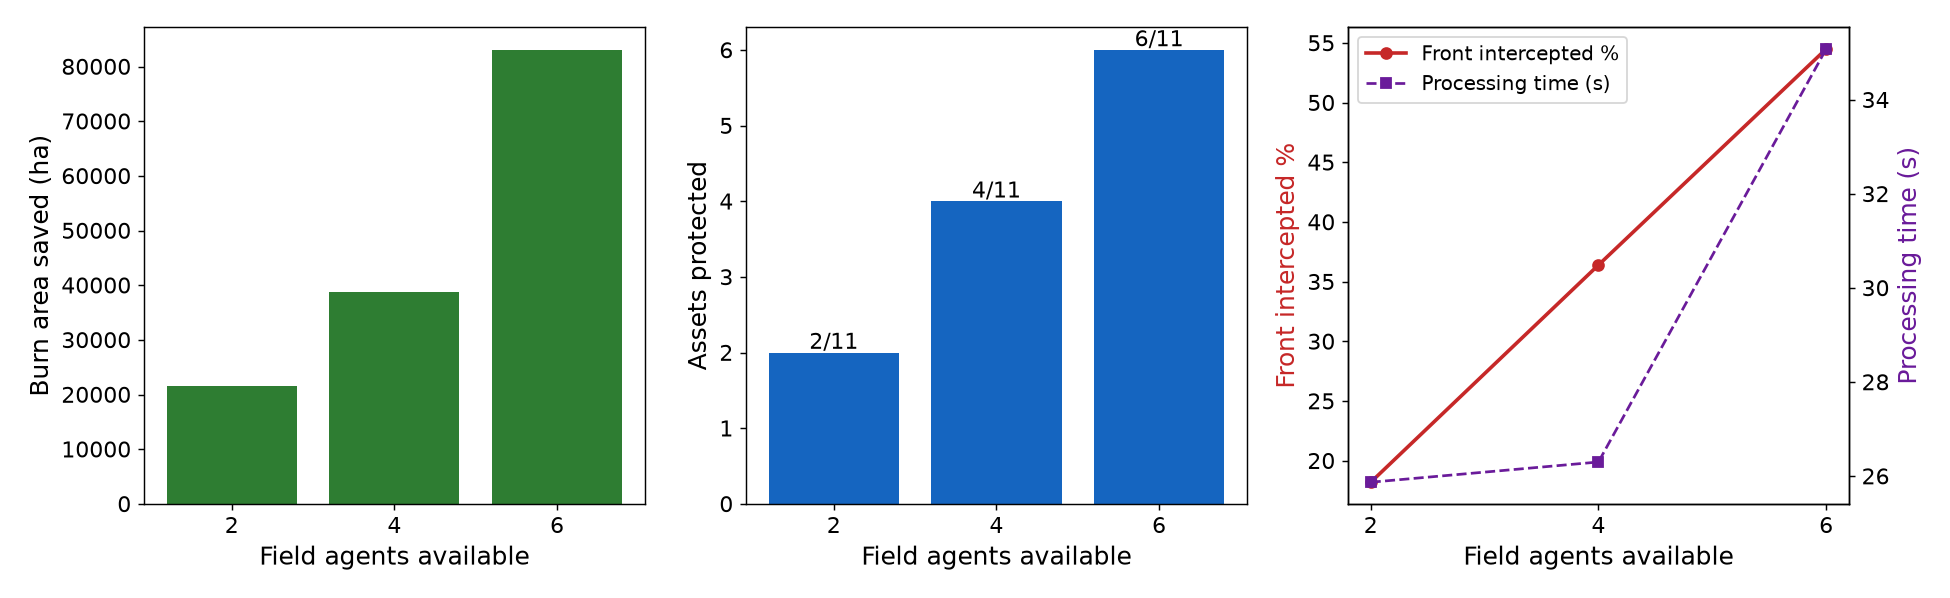
\includegraphics[width=\textwidth]{fig9_multiagent_evaluation.png}
  \caption{Multi-agent coordination results: area saved, assets protected, and fire front interception across three deployment scenarios.}
  \label{fig:agents}
\end{figure}

The results demonstrate a clear and consistent scaling benefit with additional field agents. Moving from 2 to 6 agents increases fire front interception from 18.2\% to 54.5\% and area saved from 21,642\,ha to 83,031\,ha, a 3.84$\times$ improvement in protected area despite only a 3$\times$ increase in agent count. This super-linear scaling is most pronounced in the 4-to-6 agent step (38,754\,ha to 83,031\,ha, a 2.14$\times$ jump), which is explained by the Commander Agent's ability to cover a wider angular arc of the downwind fire front when a sixth agent is added: with only four agents, the two highest-priority assets on the eastern flank of the spread cannot be simultaneously intercepted without one agent exceeding the road-network feasibility margin; the sixth agent resolves this constraint and unlocks protection of an additional 44,277\,ha. This kind of constraint-aware, route-feasibility-verified allocation is precisely what distinguishes the LLM coordination layer from a simple nearest-assignment heuristic.

Regarding processing latency, all three scenarios completed end-to-end within 36 seconds including LLM reasoning, Dijkstra route verification, and Evaluator assessment. The 4-agent scenario was marginally faster than the 6-agent scenario (26.3 s vs. 35.1 s) because the Commander's reasoning chain is longer when coordinating six independent agents and justifying a wider set of prioritisation decisions. Critically, even the 6-agent scenario's 35-second total latency is orders of magnitude faster than the hours typically required for a human incident commander to process satellite data, consult maps, assess road accessibility, and coordinate field team deployment. This confirms the practical utility of the framework for time-critical emergency response.

The Evaluator Agent independently assessed all three plans for plan robustness. In the 4- and 6-agent scenarios, all field agent assignments had feasibility margins exceeding 20 minutes (the ROBUST threshold), meaning each team would arrive at their interception point with more than 20 minutes to spare before fire arrival. In the 2-agent scenario, one assignment was flagged as FRAGILE (margin $<$ 20 minutes), triggering a Commander reassignment loop in which the Commander re-evaluated whether to accept the fragile assignment or redirect that agent to a lower-priority but more accessible asset. This self-correcting feedback loop between the Evaluator and Commander agents is a key architectural feature that improves plan reliability without requiring human intervention.

\subsection{Discussion}

The results across all five modules highlight several interconnected findings that collectively distinguish this framework from the reviewed literature. The LightGBM classifier achieves a ROC-AUC of 0.9874 and 95.6\% accuracy on the 200,000-sample Amazon dataset, comparable to Iban and Aksu~\cite{iban2024} who reported 95.6\% for Random Forest in T\"{u}rkiye and Freitas et al.~\cite{freitas2024} in the Triunfo do Xingu Protection Area. However, those studies evaluated models on datasets of at most tens of thousands of samples from single regions, whereas our benchmark spans the entire Brazilian Amazon across six years, making the generalisation guarantee substantially stronger. Tang et al.~\cite{tang2024} reported 99.6\% accuracy for XGBoost in Thailand, but their positive class was defined from satellite fire pixels rather than independently verified INPE ground records, which can introduce label noise near fire perimeters. Rub\'{i} et al.~\cite{rubi2023} achieved only 91\% using AdaBoost in the Brazilian Cerrado, below all seven of our models, likely reflecting both dataset size limitations and AdaBoost's sensitivity to noisy labels relative to gradient-boosted trees. Hang et al.~\cite{hang2024} similarly achieved AUC above 0.90 with stacking in the Western Himalaya, a strong result but on a considerably smaller and geographically narrower dataset than ours.

On the explainability side, our SHAP analysis confirms temperature and humidity as the dominant predictors (combined contribution $>$ 60\%), with Farming land cover as the third most important driver. This directly corroborates De Santana et al.~\cite{desantana2024}, who showed that distance to farming areas is the single most important Amazon fire predictor using Maxent, and aligns with Abdollahi and Pradhan~\cite{abdollahi2023}, who identified humidity and wind as top predictors in Australian wildfires. What distinguishes our approach is the combination of SHAP with LIME for instance-level validation: while both De Santana et al. and Abdollahi and Pradhan report only global feature rankings, our dual-XAI framework verifies that the model's reasoning is locally consistent at the level of individual predictions, a necessary step for building trust in operational fire alert systems.

The Rothermel-CA simulation burns 563\,ha over 12 hours with 94.1\% of the burn footprint pre-flagged as High or Very High risk by the ML model, providing cross-validation between the two pipeline components. Xu et al.~\cite{xu2022} proposed learning CA transition rules from historical fire data using LSSVM instead of embedding physical equations, which avoids manual fuel parameter calibration but requires a large historical spread dataset unavailable at the national Amazon scale. Perello et al.~\cite{perello2024} demonstrated that probabilistic CA simulators can serve as operational planning tools in Liguria, Italy, but their PROPAGATOR model is calibrated for Mediterranean shrubland and cannot be transferred to tropical Amazon conditions without extensive recalibration, whereas the Rothermel equations used here have universal physical grounding across fuel types. Furthermore, none of the reviewed spread simulation works connect their outputs to any downstream response planning layer, leaving the gap between fire prediction and field action unaddressed.

On ecological risk, all ten reviewed works produce raster susceptibility maps, but none translate those maps into named-entity risk scores tied to specific protected areas, indigenous territories, or settlements. Luz et al.~\cite{luz2022} represent the geographically closest prior work, mapping Amazon fire susceptibility from Landsat-8 and MODIS, but their output is a pure probability raster with no overlay against ICMBio or FUNAI boundaries. Our framework computes PAVI, ITRI, STS, and FVI for every named polygon, producing a ranked list of at-risk entities that can be directly handed to government agencies for prioritised monitoring and resource allocation.

The most fundamental distinction between this framework and all ten reviewed works is the multi-agent LLM coordination layer. Every reviewed paper stops at susceptibility mapping or spread simulation; none addresses how field resources should be allocated, which assets should be prioritised, or whether a response team can physically reach an interception point before the fire arrives. The three-role multi-agent system closes this gap by translating spread simulation output into a feasibility-verified, priority-ranked deployment plan within 36 seconds, with Dijkstra-based road network verification ensuring that each assignment is physically executable under real Amazon road infrastructure conditions. A limitation of the current framework is that the spread simulation is fixed to a 12-hour, 51$\times$51\,km window; fires persisting beyond this domain would require re-seeding from live NASA FIRMS detections. Future work will focus on multi-day spread chains, Monte Carlo ensemble runs for uncertainty quantification, and scaling the agent fleet to handle simultaneous multi-ignition events across the broader Legal Amazon.

% -----------------------------------------------------------------------
\section{Conclusion}
% -----------------------------------------------------------------------

This paper presented a multi-agent AI framework for Amazon forest fire detection, spread forecasting, and autonomous response coordination, addressing the critical gap between satellite-based fire monitoring and on-ground emergency action. The proposed system integrates six key components: a 200,000-sample dataset fusing six years of INPE fire records with ERA5 weather reanalysis and live Sentinel-2 and MODIS satellite imagery via Google Earth Engine; a seven-model machine learning benchmark in which LightGBM achieved a ROC-AUC of 0.9874 and 95.6\% accuracy on a held-out test set, outperforming Random Forest, CatBoost, TabNet, and ANN baselines; SHAP and LIME explainability analyses identifying temperature, humidity, and Farming land cover as the dominant fire drivers; a Rothermel physics-based cellular automata simulation at 100\,m cell resolution that burned 563\,ha over 12 hours from a Rond\^{o}nia ignition point, with 94.1\% of the burn area pre-flagged as high risk by the ML model; a GIS ecological risk overlay scoring 45,000 grid points across 143 protected areas and 351 indigenous territories, producing PAVI, ITRI, STS, and FVI indices that pinpointed nine indigenous territories and seven settlements at critical risk in the Arc of Deforestation; and a three-role LLM multi-agent coordination system (Commander, Field Agents, Evaluator) that autonomously dispatched field teams, achieving a fire front interception of 54.5\% and protecting 83,031\,ha with six field agents deployed, all within 36 seconds of end-to-end processing. The primary novelty of this work lies in closing the loop from passive fire detection to active, real-time response planning through autonomous AI agent coordination, a capability absent from all reviewed prior works. Future work will focus on extending the spread simulation to multi-day fire chains, incorporating ensemble fire weather forecasts, integrating real-time NASA FIRMS active fire feeds for dynamic re-ignition seeding, and scaling the agent fleet to handle simultaneous multi-ignition events across the broader Legal Amazon.

% -----------------------------------------------------------------------
\begin{thebibliography}{10}

\bibitem{xu2022}
Y.~Xu, D.~Li, H.~Ma, R.~Lin, and F.~Zhang,
``Modeling forest fire spread using machine learning-based cellular automata in a GIS environment,''
\textit{Forests}, vol.~13, no.~12, p.~1974, Dec.~2022,
doi: 10.3390/f13121974.

\bibitem{abdollahi2023}
A.~Abdollahi and B.~Pradhan,
``Explainable artificial intelligence (XAI) for interpreting the contributing factors feed into the wildfire susceptibility prediction model,''
\textit{Science of the Total Environment}, vol.~879, p.~163004, Jul.~2023,
doi: 10.1016/j.scitotenv.2023.163004.

\bibitem{hang2024}
H.~T.~Hang, J.~Mallick, S.~Alqadhi, A.~A.~Bindajam, and H.~G.~Abdo,
``Exploring forest fire susceptibility and management strategies in Western Himalaya: Integrating ensemble machine learning and explainable AI for accurate prediction and comprehensive analysis,''
\textit{Environmental Technology and Innovation}, vol.~35, p.~103655, Aug.~2024,
doi: 10.1016/j.eti.2024.103655.

\bibitem{iban2024}
M.~C.~Iban and O.~Aksu,
``SHAP-driven explainable artificial intelligence framework for wildfire susceptibility mapping using MODIS active fire pixels: An in-depth interpretation of contributing factors in Izmir, T\"{u}rkiye,''
\textit{Remote Sensing}, vol.~16, no.~15, p.~2842, Aug.~2024,
doi: 10.3390/rs16152842.

\bibitem{rubi2023}
J.~N.~S.~Rub\'{i}, P.~H.~P.~de~Carvalho, and P.~R.~L.~Gondim,
``Application of machine learning models in the behavioral study of forest fires in the Brazilian Federal District region,''
\textit{Engineering Applications of Artificial Intelligence}, vol.~118, p.~105649, Feb.~2023,
doi: 10.1016/j.engappai.2022.105649.

\bibitem{tang2024}
J.~Tang, M.~Weeramongkolkul, S.~Suwankesawong, K.~Saengtabtim, N.~Leelawat, and K.~Wongwailikhit,
``Toward a more resilient Thailand: Developing a machine learning-powered forest fire warning system,''
\textit{Heliyon}, vol.~10, no.~13, p.~e34021, Jul.~2024,
doi: 10.1016/j.heliyon.2024.e34021.

\bibitem{luz2022}
A.~E.~O.~Luz, R.~G.~Negri, K.~G.~Massi, M.~Colnago, E.~A.~Silva, and W.~Casaca,
``Mapping fire susceptibility in the Brazilian Amazon forests using multitemporal remote sensing and time-varying unsupervised anomaly detection,''
\textit{Remote Sensing}, vol.~14, no.~10, p.~2429, May~2022,
doi: 10.3390/rs14102429.

\bibitem{perello2024}
N.~Perello, A.~Trucchia, F.~Baghino, B.~S.~Asif, L.~Palmieri, N.~Rebora, and P.~Fiorucci,
``Cellular automata-based simulators for the design of prescribed fire plans: the case study of Liguria, Italy,''
\textit{Fire Ecology}, vol.~20, no.~1, p.~7, Jan.~2024,
doi: 10.1186/s42408-023-00239-7.

\bibitem{freitas2024}
K.~M.~Freitas, R.~S.~Juvanhol, C.~J.~G.~Pinheiro, and A.~A.~de~M.~Meneses,
``Prediction of forest fire susceptibility using machine learning tools in the Triunfo do Xingu Environmental Protection Area, Amazon, Brazil,''
\textit{SSRN preprint}, 2024,
doi: 10.2139/ssrn.5039001.

\bibitem{desantana2024}
M.~M.~M.~de~Santana, R.~N.~de~Vasconcelos, E.~Mariano~Neto, and W.~de~J.~S.~da~Franca~Rocha,
``Machine learning model reveals land use and climate's role in Amazon wildfires: Present and future scenarios,''
\textit{Fire}, vol.~7, no.~10, p.~338, Oct.~2024,
doi: 10.3390/fire7100338.

\end{thebibliography}

\end{document}
